\documentclass[10pt,a4paper]{article}
\usepackage[margin=1.8cm]{geometry}
\usepackage[T1]{fontenc}
\usepackage{lmodern}
\usepackage{booktabs,graphicx,xcolor,multicol,enumitem,titlesec,array}
\usepackage[hidelinks]{hyperref}
\definecolor{navy}{HTML}{1F3A5F}
\titleformat{\section}{\color{navy}\large\bfseries}{\thesection}{0.6em}{}
\titlespacing*{\section}{0pt}{8pt}{3pt}
\setlist{nosep,leftmargin=1.2em}
\setlength{\parindent}{0pt}
\setlength{\parskip}{4pt}
\hypersetup{pdftitle={ICICI Bank initiation}, pdfauthor={Vinayak Singh}}
\begin{document}

{\color{navy}\rule{\linewidth}{2pt}}\\[-2pt]
{\Large\bfseries ICICI Bank Ltd (NSE: ICICIBANK)}\hfill{\small Initiation of coverage, 1 Nov 2026}\\[2pt]
{\large Growth is back, but margins and valuation cap the upside}\\[-4pt]
{\color{navy}\rule{\linewidth}{0.6pt}}


\begin{minipage}[t]{0.33\linewidth}
\vspace{0pt}
\fcolorbox{navy}{navy!6}{\begin{minipage}{0.92\linewidth}\small
\textbf{Rating: HOLD}\\[2pt]
12-month target: \textbf{Rs 1,353}\\
Price (23 Oct 2026): Rs 1,394.2\\
Implied return: -2.9\%\\[4pt]
Bull / bear value: Rs 1,633 / Rs 891\\[4pt]
Market cap: Rs 9.98 trn\\
Shares: 7.16 bn\\
P/B FY27E: 2.58x\\
P/E FY27E: 17.1x\\
Cost of equity: 12.4\%\\
Long-run growth: 8.0\%\\
Price change, 1y: 2\%\\
Price change, 3y: 50\%
\end{minipage}}

\smallskip
{\footnotesize Analyst: Vinayak Singh, IIT Kharagpur\\ Student research for learning purposes; not investment advice.}
\end{minipage}\hfill
\begin{minipage}[t]{0.63\linewidth}
\vspace{0pt}\small
\textbf{Investment summary}
\begin{itemize}
\item \textbf{Five years of strong delivery.} Profit after tax compounded 21\% a year from FY22 to FY26 (Rs 233 bn to Rs 501 bn) as loans grew 16\% a year, gross NPAs fell from 3.60\% to 1.40\% and ROE peaked at 18.6\% in FY24.
\item \textbf{H1 FY27: fast growth, thinner margin.} Profit rose 18\% year on year in the first half. Loans grew 30.0\% year on year, but 24.1\% excluding loans that international branches made against FCNR(B) (foreign-currency) deposits, which also lifted deposit growth from 17.0\% to 27.1\%. NIM fell to 4.18\% in Q2, from 4.53\% in FY24.
\item \textbf{Fair value close to the price.} Our base case has ROE of 16.1--15.8\% over FY27E--FY29E and EPS growth of 14\% a year. A residual income model at a 12.4\% cost of equity values the standalone bank at Rs 1,194 in 12 months; listed subsidiaries add Rs 159 after a 20\% discount, for a target of Rs 1,353. The price implies a cost of equity of 11.9\% or perpetual growth of 9.0\%.
\item \textbf{What would change our view:} NIM recovering above 4.3\% with growth above 15\%, or credit costs staying near 0.3\% through FY29 (bull case Rs 1,633); a credit cycle would take value to Rs 891.
\end{itemize}
\end{minipage}

\medskip
\begin{center}\small
\textbf{Key financials (standalone, base case)}\\[2pt]
\begin{tabular}{lrrrrr}
\toprule
 & FY25A & FY26A & FY27E & FY28E & FY29E \\
\midrule
Net interest income (Rs bn) & 812 & 881 & 1,004 & 1,187 & 1,374 \\
Core operating profit (Rs bn) & 654 & 704 & 825 & 964 & 1,110 \\
Provisions (Rs bn) & 47 & 54 & 52 & 92 & 117 \\
Profit after tax (Rs bn) & 472 & 501 & 584 & 659 & 750 \\
EPS (Rs) & 66.3 & 70.0 & 81.5 & 92.0 & 104.7 \\
EPS growth (\%) & 13.9 & 5.7 & 16.4 & 12.8 & 13.9 \\
Book value per share (Rs) & 410 & 471 & 541 & 619 & 708 \\
Net interest margin (\%) & 4.32 & 4.32 & 4.20 & 4.20 & 4.25 \\
Cost-to-income, core (\%) & 39.3 & 40.2 & 38.5 & 38.5 & 38.5 \\
Credit cost (\%) & 0.37 & 0.37 & 0.30 & 0.45 & 0.50 \\
ROA (\%) & 2.37 & 2.23 & 2.22 & 2.12 & 2.11 \\
ROE (\%) & 17.8 & 15.9 & 16.1 & 15.9 & 15.8 \\
\midrule
P/E at Rs 1,394 (x) & 21.0 & 19.9 & 17.1 & 15.2 & 13.3 \\
P/B at Rs 1,394 (x) & 3.40 & 2.96 & 2.58 & 2.25 & 1.97 \\
\bottomrule
\end{tabular}
\end{center}
{\footnotesize Source: ICICI Bank results presentations and audited results FY22--FY26 (see Appendix); FY27E--FY29E are our estimates. ROE is our calculation on average net worth; the bank reports 16.0\% for FY26.}

\newpage
\section{Five years of re-rating: what drove earnings}
\begin{minipage}[t]{0.5\linewidth}\vspace{0pt}
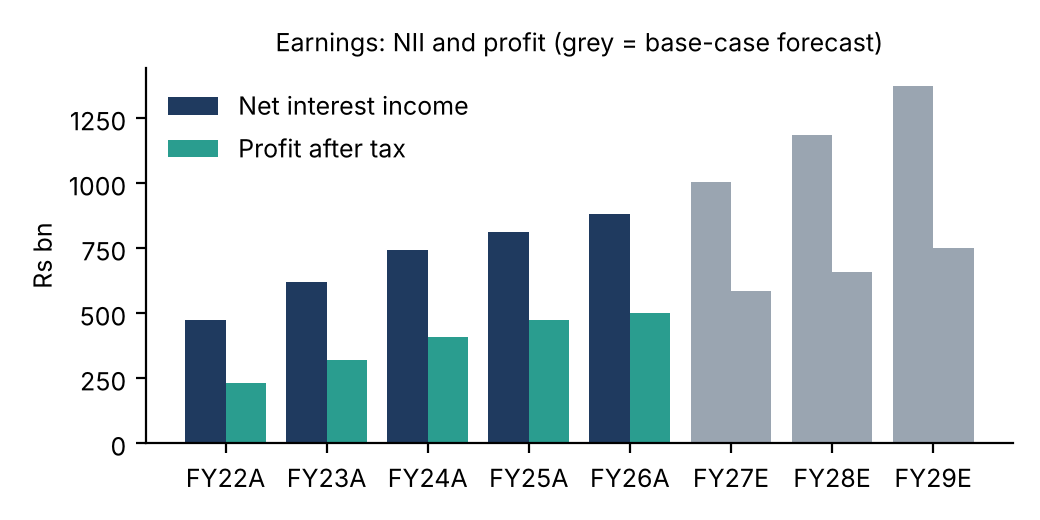
\includegraphics[width=\linewidth]{../charts/earnings.png}
\end{minipage}\hfill
\begin{minipage}[t]{0.47\linewidth}\vspace{0pt}\small
Net interest income nearly doubled from Rs 475 bn in FY22 to Rs 881 bn in FY26, while operating expenses grew more slowly, from Rs 267 bn to Rs 472 bn, so core cost-to-income eased from 41.1\% to 40.2\%.

The bigger swing was provisions: Rs 86 bn in FY22 against Rs 54 bn in FY26, even though the loan book was 1.8 times larger. Lower credit costs explain much of the jump in ROA from 1.84\% to 2.37\%.

Profit growth has slowed sharply: 37\% in FY23, 28\% in FY24, 16\% in FY25 and 6\% in FY26. FY26 provisions included a one-off Rs 12.8 bn standard-asset provision directed by the RBI.
\end{minipage}

\begin{minipage}[t]{0.5\linewidth}\vspace{0pt}
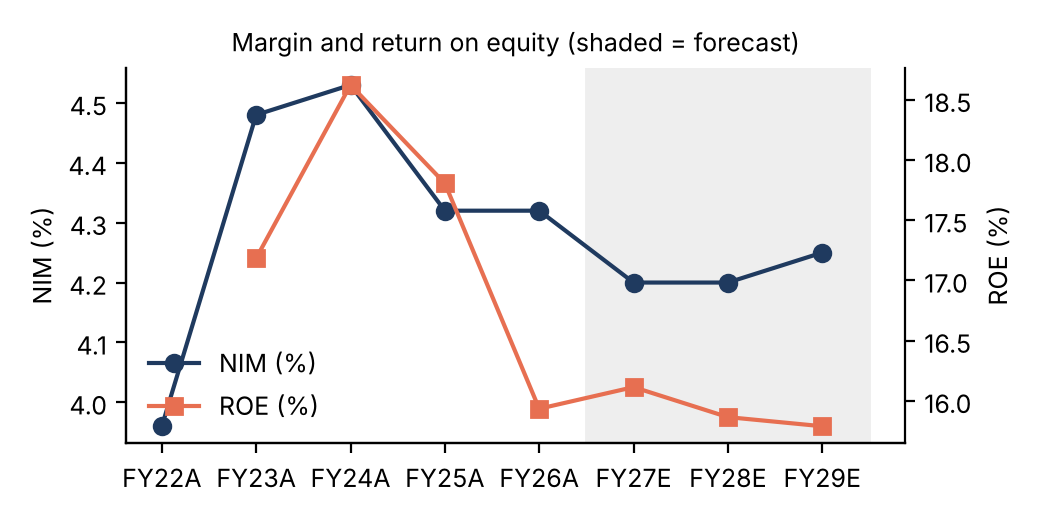
\includegraphics[width=\linewidth]{../charts/nim_roe.png}
\end{minipage}\hfill
\begin{minipage}[t]{0.47\linewidth}\vspace{0pt}\small
\textbf{Margin.} NIM peaked at 4.53\% in FY24 as loans repriced faster than deposits after the 2022--23 rate hikes. Since then deposit costs have caught up, and the share of CASA (current and savings accounts, the cheapest funding) in period-end deposits has fallen from 48.7\% in FY22 to 41.4\% in FY26 and 36.1\% in September 2026.

\textbf{Returns.} ROE on our basis fell from 18.6\% in FY24 to 15.9\% in FY26: margins slipped, credit costs normalised a little, and equity built up faster than profit (CET1 16.35\% in FY26, well above requirements). Surplus capital lowers ROE but gives room to grow.
\end{minipage}

\begin{minipage}[t]{0.5\linewidth}\vspace{0pt}
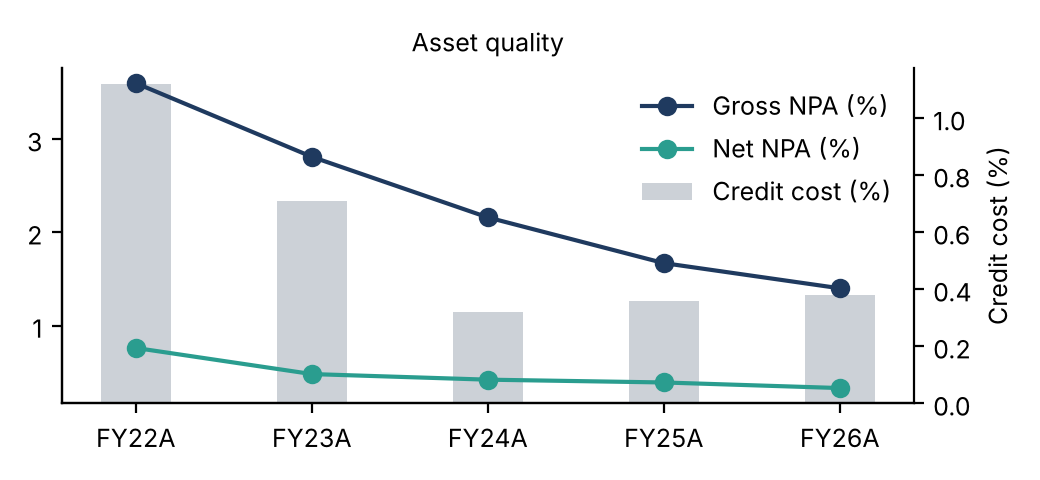
\includegraphics[width=\linewidth]{../charts/asset_quality.png}
\end{minipage}\hfill
\begin{minipage}[t]{0.47\linewidth}\vspace{0pt}\small
\textbf{Asset quality.} Gross NPAs fell every year, from 3.60\% to 1.40\% (and 1.20\% in September 2026); net NPAs are only 0.33\%. Provision coverage has slipped from 82.8\% (FY23) to 75.8\%, which is still high.

With credit costs at 0.32--0.38\%, there is little left to gain from here. Our base case lets credit costs rise to 0.50\% by FY29E, close to a through-the-cycle level for a lender with this mix.
\end{minipage}

\section{First half of FY27: what changed}
\small Net interest income grew 15.2\% and operating expenses 9.4\% year on year in H1 FY27, so profit after tax rose 18.0\% to Rs 296 bn. Provisions were only Rs 21 bn (credit cost 0.25\% annualised).

The balance sheet changed shape. Loans rose from Rs 15,539 bn in March to Rs 18,316 bn in September, and deposits from Rs 17,946 bn to Rs 20,499 bn. Much of the increase was foreign-currency FCNR(B) deposits lent on by the bank's international branches: excluding them, loans grew 24.1\% and deposits 17.0\% year on year, against 30.0\% and 27.1\% including them. The presentation does not give the margin on this book, but NIM fell from 4.36\% in Q1 to 4.18\% in Q2 as it grew, which suggests it earns less than the rest of the balance sheet. We treat it as lower-margin growth: our FY27E loan growth of 22\% includes it, and our NIM of 4.20\% assumes the second half stays near the Q2 level.

\clearpage\section{Forecasts: three scenarios}
\small Loans and total assets grow at the scenario rate. Net interest income is NIM times average interest-earning assets, which we hold at the FY26 ratio of 90.8\% of average total assets (implied by reported NII and NIM). Operating expenses follow core cost-to-income, provisions follow credit cost on average loans, and dividends follow the payout ratio, paid the following year. Treasury gains are not forecast.

\begin{center}\footnotesize
\resizebox{\linewidth}{!}{\begin{tabular}{lrrrrrrrrr}
\toprule
 & \multicolumn{3}{c}{Bear} & \multicolumn{3}{c}{Base} & \multicolumn{3}{c}{Bull} \\
\cmidrule(lr){2-4}\cmidrule(lr){5-7}\cmidrule(lr){8-10}
 & FY27E & FY28E & FY29E & FY27E & FY28E & FY29E & FY27E & FY28E & FY29E \\
\midrule
Loan growth (\%) & 19.0 & 11.0 & 11.0 & 22.0 & 15.0 & 14.0 & 25.0 & 18.0 & 16.0 \\
Net interest margin (\%) & 4.10 & 4.00 & 4.00 & 4.20 & 4.20 & 4.25 & 4.27 & 4.35 & 4.40 \\
Non-interest income growth, ex treasury (\%) & 10.0 & 9.0 & 9.0 & 14.0 & 13.0 & 13.0 & 15.0 & 15.0 & 15.0 \\
Cost-to-income, core (\%) & 39.5 & 40.5 & 40.5 & 38.5 & 38.5 & 38.5 & 38.0 & 37.5 & 37.5 \\
Credit cost, provisions / avg loans (\%) & 0.40 & 0.90 & 0.80 & 0.30 & 0.45 & 0.50 & 0.25 & 0.35 & 0.40 \\
Tax rate (\%) & 24.5 & 24.5 & 24.5 & 24.5 & 24.5 & 24.5 & 24.5 & 24.5 & 24.5 \\
Dividend payout (\%) & 17.0 & 17.0 & 17.0 & 17.0 & 17.0 & 17.0 & 17.0 & 17.0 & 17.0 \\
\midrule
Profit after tax (Rs bn) & 539 & 513 & 582 & 584 & 659 & 750 & 611 & 731 & 850 \\
ROE (\%) & 15.0 & 12.7 & 13.0 & 16.1 & 15.9 & 15.8 & 16.8 & 17.4 & 17.4 \\
12-month value (Rs) & \multicolumn{3}{c}{891} & \multicolumn{3}{c}{\textbf{1,353}} & \multicolumn{3}{c}{1,633} \\
\bottomrule
\end{tabular}}
\end{center}

\section{Valuation: residual income, sum of the parts}
\small A bank's value comes from the return it earns on equity above its cost of equity. The residual income model makes this explicit: value = book value today + present value of (profit $-$ cost of equity $\times$ opening book). We use a 12.4\% cost of equity (India 10-year bond yield 7.40\% on 30 Oct 2026, beta 1.0, equity risk premium 5.0\%) and 8.0\% long-run growth of residual income after FY29E.

\begin{minipage}[t]{0.48\linewidth}\vspace{0pt}\footnotesize
\textbf{Residual income valuation (base case)}\\[2pt]
\begin{tabular}{lr}
\toprule
Net worth, 31 Mar 2026 (Rs bn) & 3,374 \\
Residual income FY27E (Rs bn) & 165 \\
Residual income FY28E (Rs bn) & 178 \\
Residual income FY29E (Rs bn) & 200 \\
PV of FY27E--FY29E residual income (Rs bn) & 430 \\
PV of terminal value (Rs bn) & 3,466 \\
Standalone value per share, 31 Mar 2026 (Rs) & 1,015 \\
Standalone value per share today (Rs) & 1,075 \\
Standalone value in 12 months (Rs) & 1,194 \\
Listed subsidiaries after 20\% discount (Rs/share) & 159 \\
\textbf{12-month target price (Rs)} & 1,353 \\
\bottomrule
\end{tabular}
\end{minipage}\hfill
\begin{minipage}[t]{0.48\linewidth}\vspace{0pt}\footnotesize
\textbf{Sensitivity of the 12-month target (Rs)}\\[2pt]
{\setlength{\tabcolsep}{4pt}\begin{tabular}{lrrrrr}
\toprule
COE $\downarrow$ / growth $\rightarrow$ & 7.0\% & 7.5\% & 8.0\% & 8.5\% & 9.0\% \\
\midrule
11.0\% & 1,628 & 1,754 & 1,921 & 2,155 & 2,506 \\
11.5\% & 1,462 & 1,551 & 1,666 & 1,819 & 2,033 \\
12.0\% & 1,330 & 1,394 & 1,475 & 1,579 & 1,717 \\
12.5\% & 1,221 & 1,269 & 1,326 & 1,399 & 1,492 \\
13.0\% & 1,131 & 1,166 & 1,208 & 1,259 & 1,323 \\
\bottomrule
\end{tabular}}

\medskip
\textbf{Cross-check: justified price-to-book}\\
Sustainable ROE (avg FY28E--FY29E): 15.8\%\\
Justified P/B = (ROE $-$ g)/(COE $-$ g) = 1.78x\\
On book value in 12 months (Rs 586), plus subsidiaries: Rs 1,202
\end{minipage}

\medskip
\textbf{Listed subsidiaries at market value.} ICICI Bank owns just over half of three listed companies. We value them at market prices on 23 Oct 2026 with a 20\% holding-company discount. Unlisted subsidiaries (ICICI Securities, ICICI Bank UK and Canada, ICICI Home Finance) are left at zero, which is conservative: one broker values all subsidiaries at about Rs 300 per share.

\begin{center}\footnotesize
\begin{tabular}{lrrrr}
\toprule
Subsidiary & Shares held (m) & Price (Rs) & Value (Rs bn) & Rs/ICICI share \\
\midrule
ICICI Life Insurance (ex ICICI Prudential Life) & 767 & 422.2 & 324 & 45 \\
ICICI Lombard General Insurance & 256 & 1,592.0 & 407 & 57 \\
ICICI Prudential AMC & 262 & 2,651.8 & 695 & 97 \\
\midrule
Total, before discount & & & 1,425 & 199 \\
After 20\% holding-company discount & & & & 159 \\
\bottomrule
\end{tabular}
\end{center}

\begin{minipage}[t]{0.5\linewidth}\vspace{0pt}
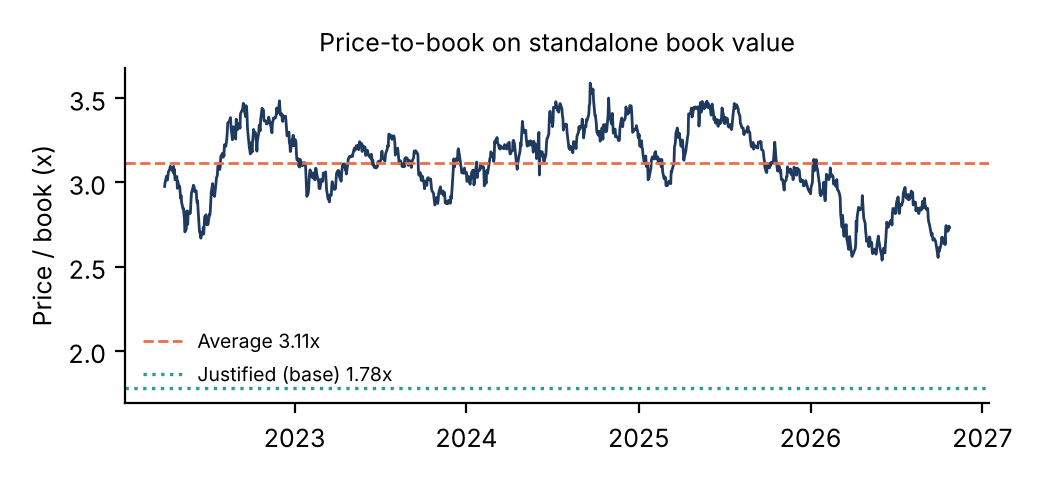
\includegraphics[width=\linewidth]{../charts/pb_band.png}
\end{minipage}\hfill
\begin{minipage}[t]{0.47\linewidth}\vspace{0pt}\small
\textbf{What the price implies.} Since FY22 the stock has traded at 2.5--3.6x standalone book (average 3.11x); today it is 2.73x. Stripping out our subsidiary value, the core bank trades at 2.62x FY26 book. Holding growth at 8\%, the current price is justified only by a cost of equity of about 11.9\%; holding the cost of equity at 12.4\%, it needs perpetual growth of about 9.0\%.

Brokers' targets after Q2 FY27 are higher than ours (Rs 1,710--2,025), mostly because they apply 2.4--2.6x to adjusted book value. The difference with our view is the assumed sustainable ROE and cost of equity, not the quality of the bank.
\end{minipage}

\section{Risks to our view}
\begin{multicols}{2}\small
\textbf{Upside risks}
\begin{itemize}
\item Faster loan growth with stable margins: the bull case (loan growth 25\% in FY27E, NIM recovering to 4.40\%) gives Rs 1,633.
\item Credit costs staying at the FY24--26 low of about 0.3--0.4\%.
\item A higher value for the unlisted subsidiaries, which we leave at zero.
\item Rate cuts, which would lower the 10-year yield and the cost of equity: each 0.5 point off the cost of equity adds roughly Rs 149 to the target.
\end{itemize}
\columnbreak
\textbf{Downside risks}
\begin{itemize}
\item Deposit competition: CASA is falling and deposit costs could squeeze NIM further.
\item A credit cycle in unsecured retail or small business loans: the bear case (credit cost up to 0.9\%) gives Rs 891.
\item Bond yields near 7.4\% and oil above \$100 raise the cost of equity and the risk of slower growth.
\item Regulatory actions, such as the RBI-directed provision taken in FY26.
\end{itemize}
\end{multicols}

\begin{minipage}[t]{0.5\linewidth}\vspace{0pt}
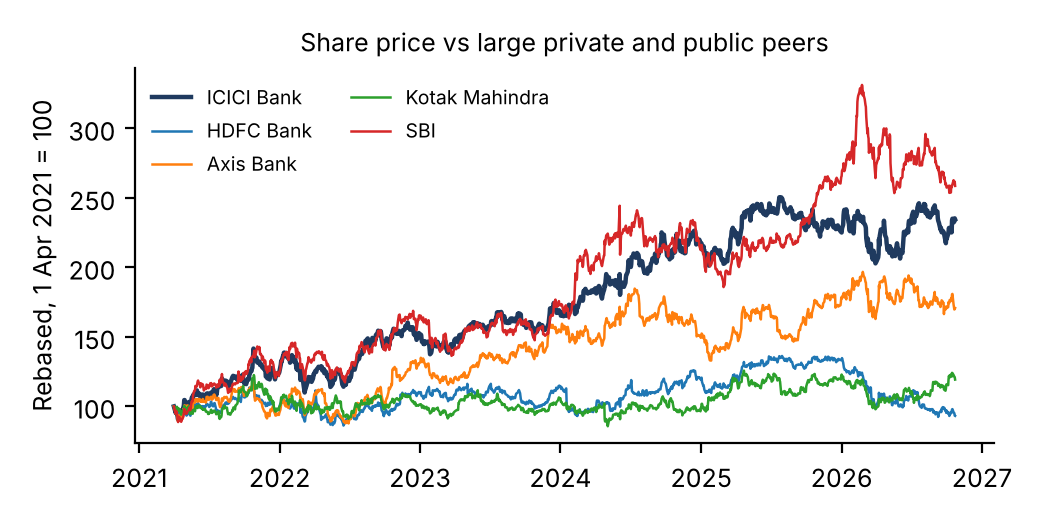
\includegraphics[width=\linewidth]{../charts/price_vs_peers.png}
\end{minipage}\hfill
\begin{minipage}[t]{0.47\linewidth}\vspace{0pt}\small
\textbf{Share price performance.} Over three years ICICI Bank returned 50\%, ahead of HDFC Bank (-8\%), Axis (26\%) and Kotak (24\%), and behind SBI (73\%). Over the past year it is up 2\%. The market already rewards ICICI as the best-run large private bank, which is why we think the stock needs returns to rise, not just hold, to beat the market from here.
\end{minipage}

\section*{Appendix: method, data and limitations}
\footnotesize
\begin{itemize}
\item \textbf{Data.} Standalone figures from ICICI Bank's Q4 investor presentations, audited results and press releases for FY22--FY26, and the Q2 FY27 results filing (17 Oct 2026). Share prices: NSE daily closes to 2026-10-23. Subsidiary stakes: Sep 2026 shareholding disclosures; ICICI Lombard form NL-9. 10-year yield: Trading Economics, 30 Oct 2026.
\item \textbf{Reproducibility.} The Python pipeline extracts the figures from the filings, rebuilds the Excel model (scenario switch, live formulas) and regenerates this report. A check recalculates the workbook and confirms it matches the Python model to six significant figures, with reported profit before tax reconciling for all five years.
\item \textbf{Limitations.} Standalone bank only; subsidiaries enter at market value. Net worth is capital plus reserves (excluding revaluation reserves), not the RBI definition. Forecasts are annual, with no quarterly seasonality. ROE is on our own basis.
\item This is a student research exercise and not a recommendation to buy or sell any security.
\end{itemize}

\end{document}
